\chapter{Materials and methods}
After analyzing some previous works on the topic and taking a look at the hardware at disposal, in this chapter, I present the work I carried out to develop the final system, composed of all the sensors streaming data synchronized in time. In particular, the focus is on:
\begin{itemize}
    \item Firmware development for the ST sensor nodes
    \item Python client development for the computer hub
    \item MATLAB script development for data processing
\end{itemize}
Figure \ref{fig:system-block-diag} is a block diagram to represent the entire system I developed. Each device, represented by a coloured rectangle, is shown with the software/firmware components built for it. Figure \ref{fig:system-flow} is another block diagram, that represents (in an higher abstraction level) the flow of operation of the system. Sensor boards can recognize motion, temperature, pressure and other data, and send them via BLE to a Linux Computer acting as the client. On the client, a Python script is responsible of fetching data while keeping data synchronized in time, while some MATLAB scripts can reorganize all the data, represent and analyze them. 

The chapter contains the implementation details of the solution, and the tools used for the process are reported at the end of it .

    \begin{figure}[ht!]
        \centering
        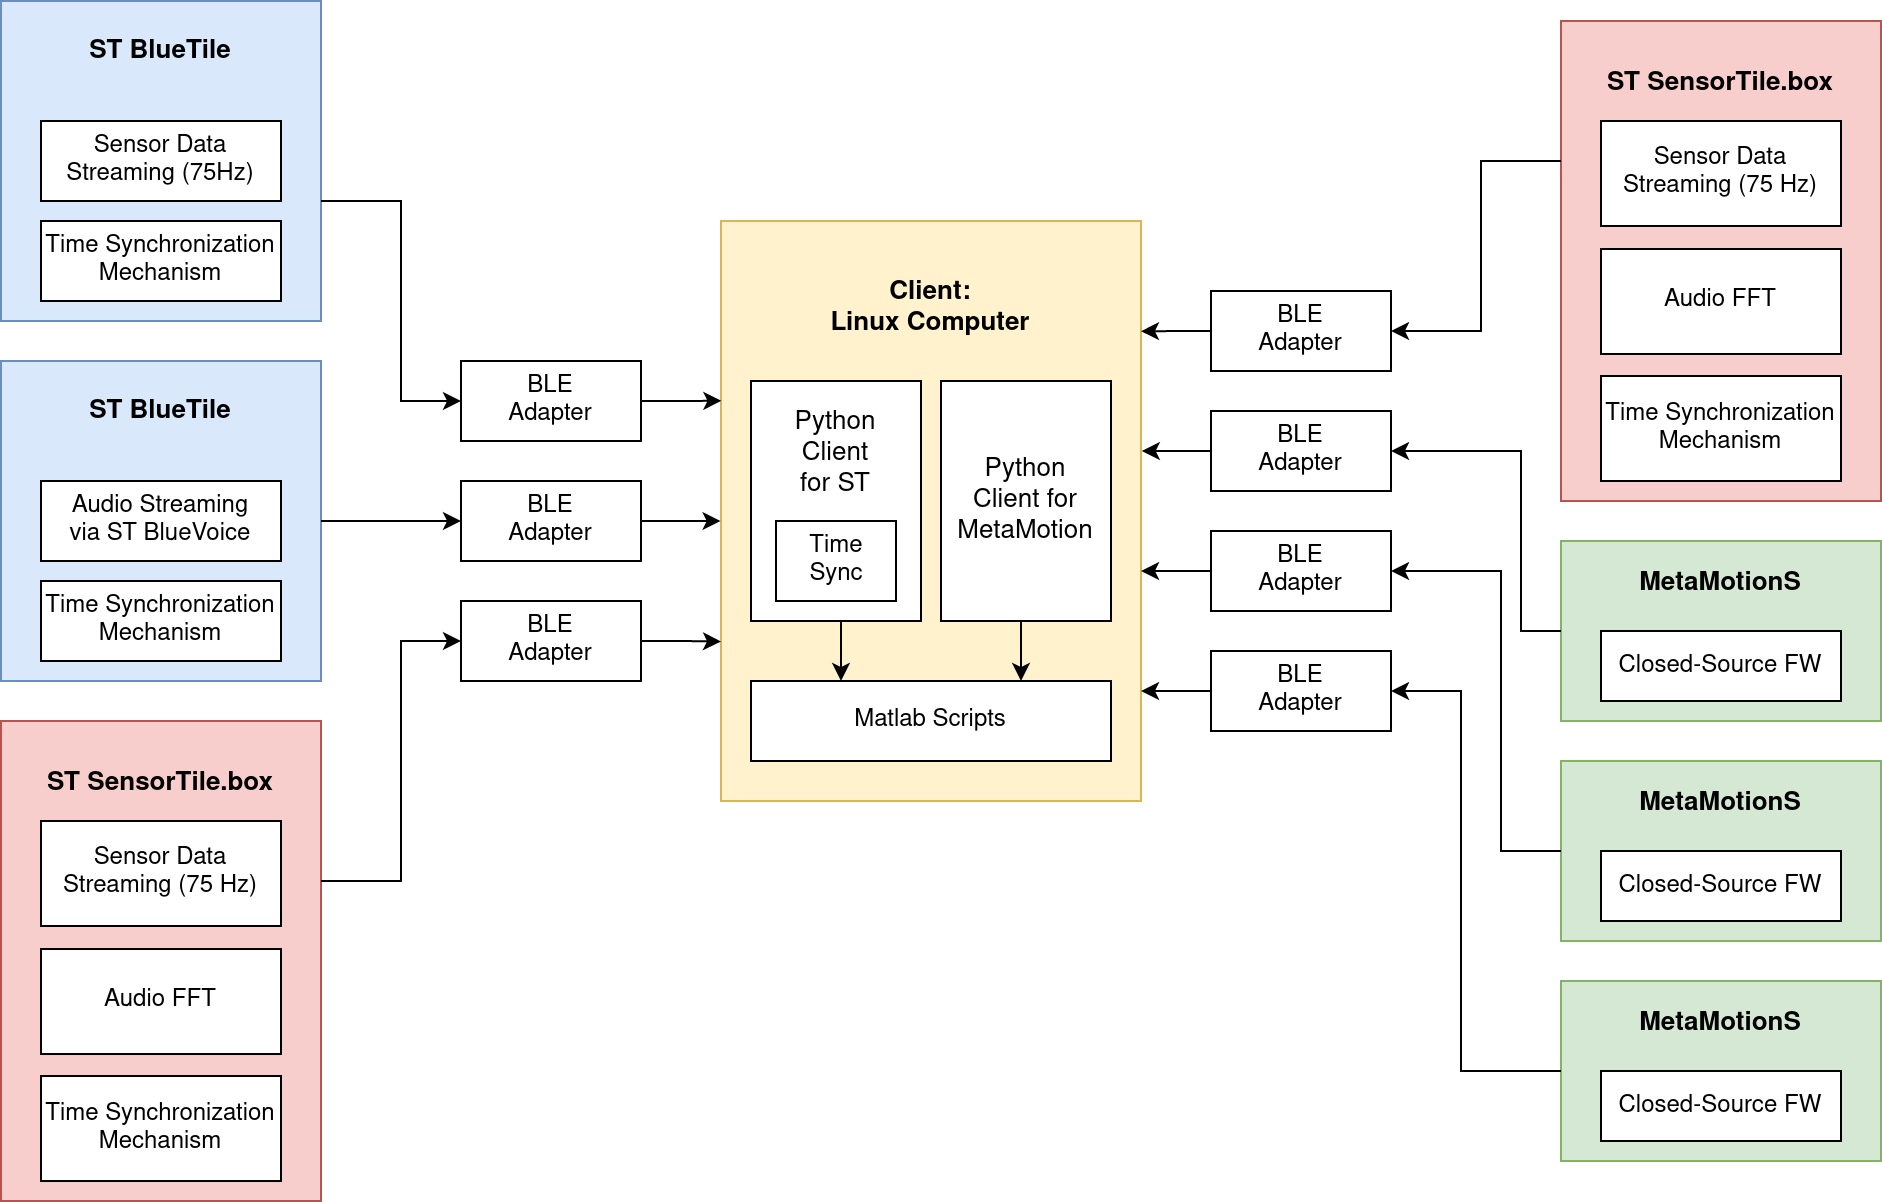
\includegraphics[width=0.85\textwidth]{chap3/figure/System_Diagram(1).png}
        \caption{Block diagram representing the developed system.}
        \label{fig:system-block-diag}
    \end{figure}

    \begin{figure}[ht!]
        \centering
        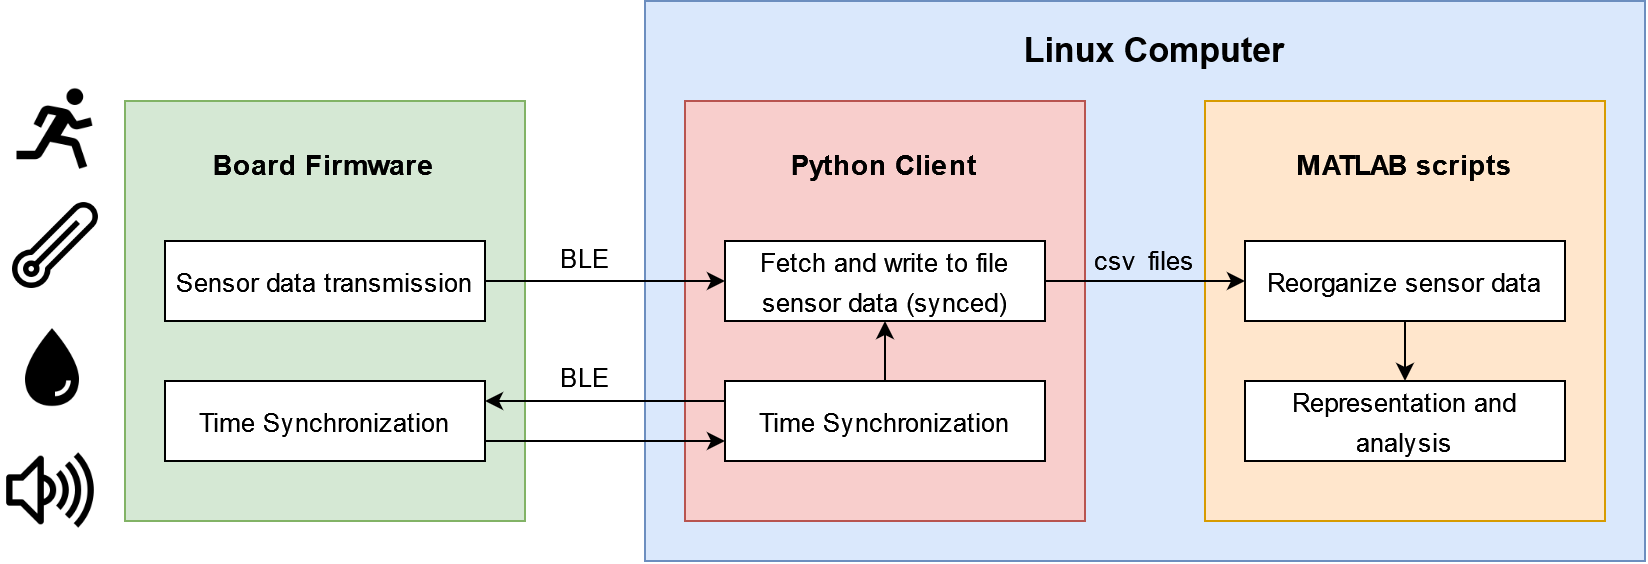
\includegraphics[width=0.85\textwidth]{chap3/figure/flow.png}
        \caption{Block diagram representing the flow of operation of the system.}
        \label{fig:system-flow}
    \end{figure}

\section{Firmware for ST devices}
%The most time-consuming part of the work has been the development of the firmware for ST devices. Despite of all the documentation and examples available on the internet, dealing with these platforms (including the BLE stack) required some in-depth study of the standards, of the implementation in the ST development environment and some trial and error to get the wanted features for the project. I've done different trials for each device, in some cases starting from scratch, in some cases starting from the available examples, exploring different possibilities and then choosing the best performing one for my goals.  
First of it all, I needed to replace the original firmware on the ST boards, applying the required modifications (for example, the data rate). Examples and documentation on the Internet have been a good starting point: then, thanks to a step-by-step approach, I wrote and built the final firmwares for all the boards, keeping in mind both the desired functionalities and the devices limitations. 

\subsection{ST BlueTile, sensing firmware}
The first board I've worked on has been the ST BlueTile one, because of its simpler configuration. In particular, I used the original firmware, called \textit{SensorDemo} \cite{bluetilesdk}, as a base for further development: in this way, the compatibility with the ST application is maintained.

The behavior of the base software is explained in Figure \ref{fig:bluetile-firmware}. It consists in a main loop, on the left part of the flowchart: at each execution, the value of some flag variables is checked and the corresponding event is executed. For example, if the variable \textit{imuTimer\_expired} is 1, it is reset and the value of the motion sensors is sent to the Bluetooth Low Energy stack for transmission. The value of these flag variables is set asynchronously by some interrupt procedures (in rectangles), that are triggered by specific events. For example, a set of hardware timers (Env Timer and Imu Timer) is configured to publish sensor and environmental data at specific rates, while other procedures will manage the behaviour at Bluetooth connection/disconnection. 

    \begin{figure}[ht!]
        \centering
        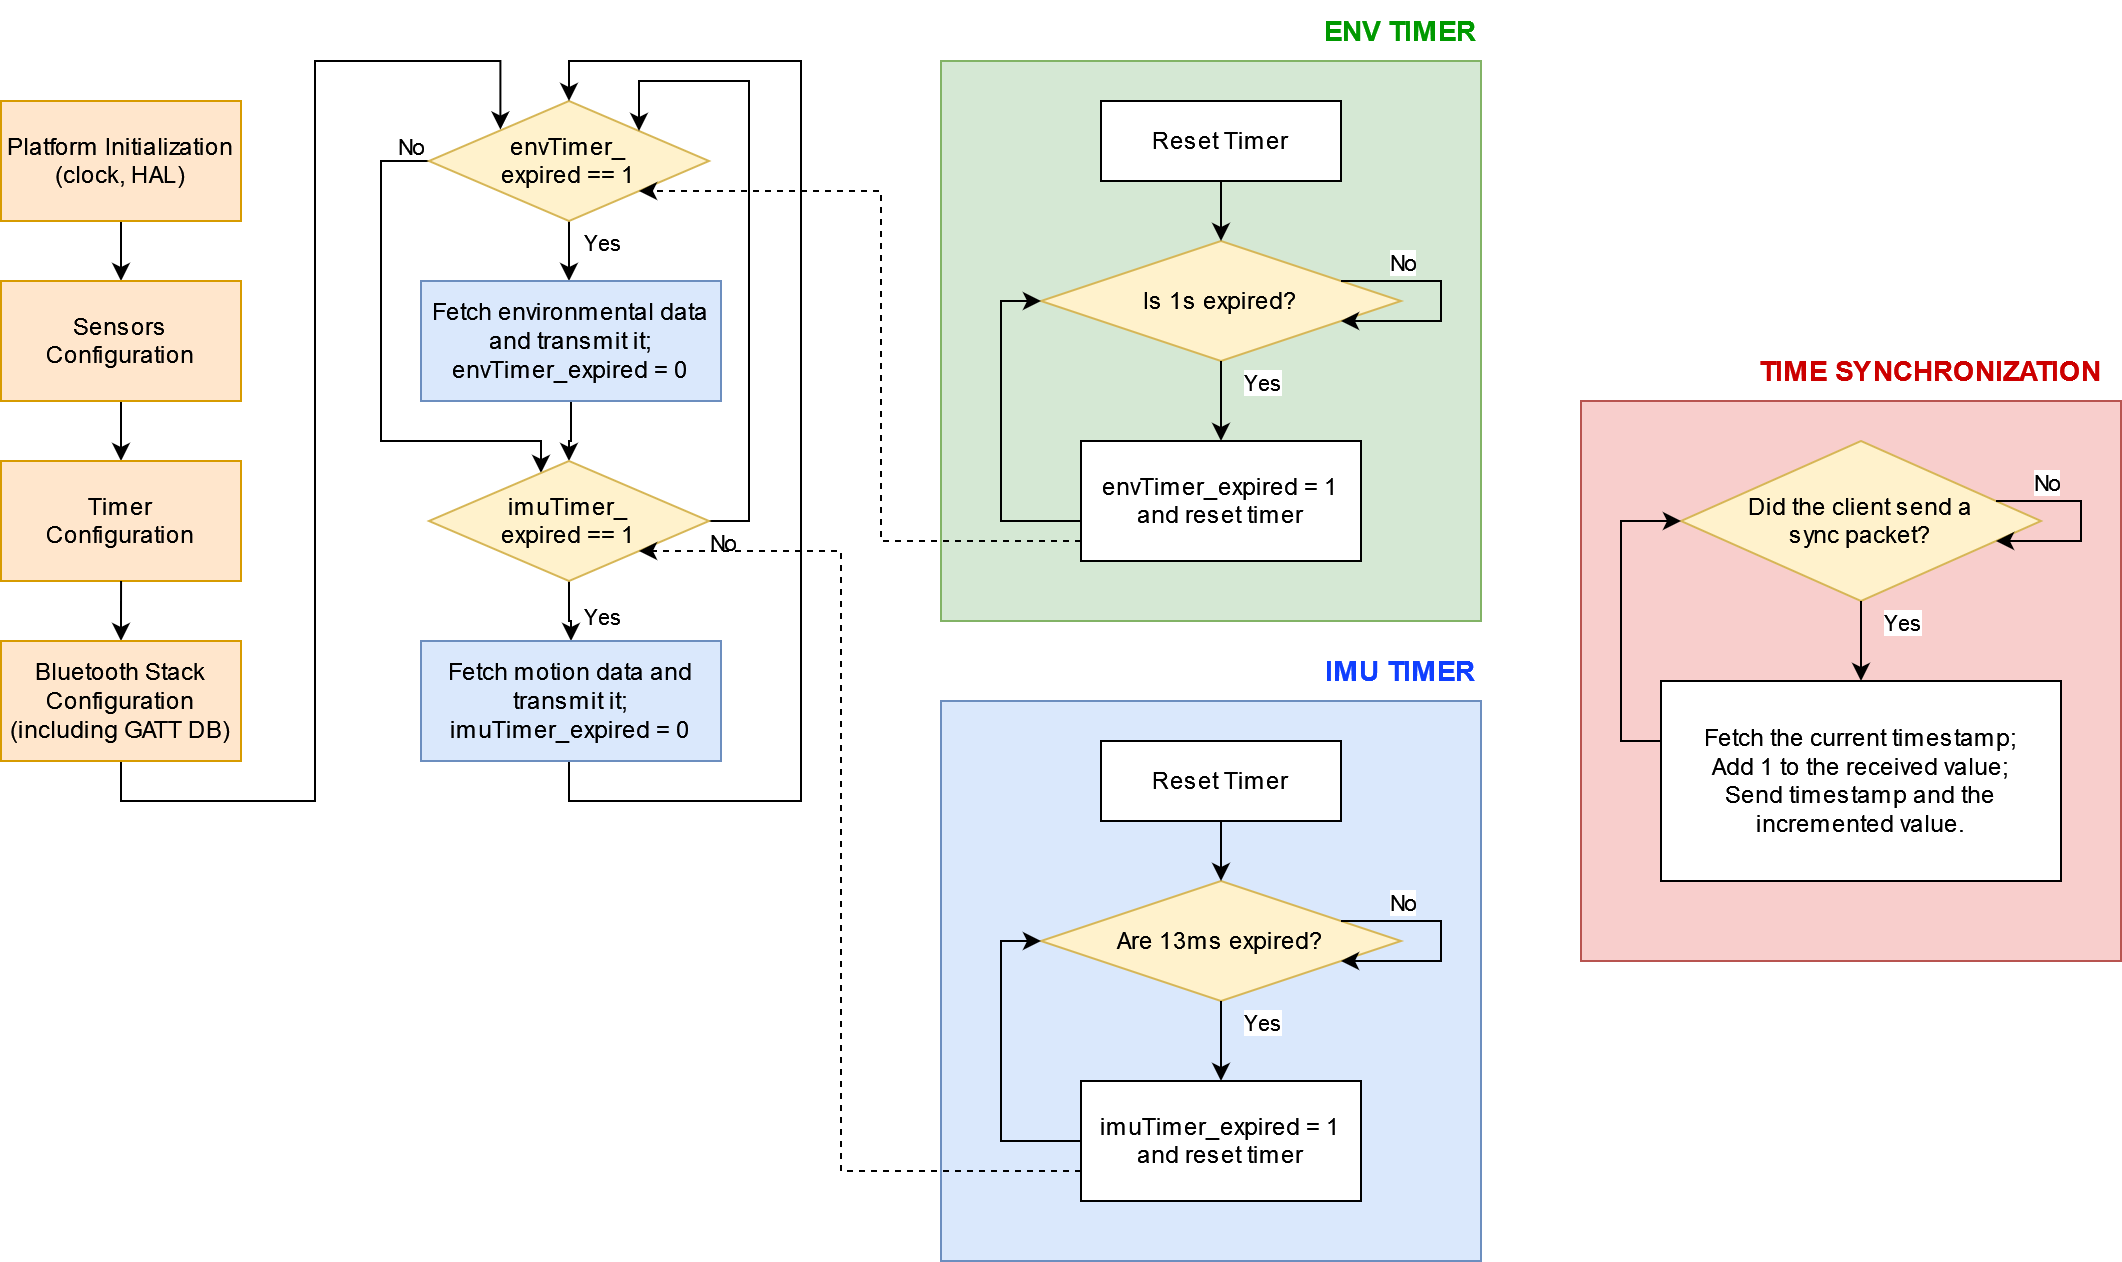
\includegraphics[width=0.85\textwidth]{chap3/figure/BlueTileFlow.png}
        \caption{Flowchart of the firmware for the BlueTile that streams sensor data.}
        \label{fig:bluetile-firmware}
    \end{figure}

The \textit{SensorDemo} firmware also contains the \textit{ST BlueVoice} library, that allows the streaming of compressed sound via Bluetooth Low Energy, optimized for voice transmission.  
I'm explaining the firmware functionalities in the following list, underlining the differences from the original one:
\begin{itemize}
    \item \textbf{Sensor data readings}. The information chosen to be transmitted to the client are the IMU (accelerometer, gyroscope, magnetometer), pressure, humidity and temperature sensors. 
    \item \textbf{Data rate modification}. I modified the rate at which IMU sensor data is transmitted over Bluetooth from 25~Hz to 75~Hz (in the last version of the firmware). Some intermediate tests have been done with other frequencies, in order to find the best one, with the corresponding results reported in the Results chapter. To perform this task, I modified the intervals of the timers which trigger sensor data updates accordingly. The rate for environmental sensor data has been lowered from 2Hz to 1Hz. 
    \item \textbf{Timestamping}. The sensor data is timestamped at the moment in which the sensor is read, and immediately before sending the packet to the BLE stack. The \textit{getTimestamp} function returns the number of milliseconds elapsed since the board power up.
    \item \textbf{BlueVoice disabled}. Even if no audio streaming is enabled, leaving \textit{BlueVoice} enabled on the small Cortex-M0 processor of the BlueTile causes some important performance degradation in sensor data streaming. This is due to some interrupts that are remaining active for audio data processing and, eventually, activation of the audio streaming functionality. For these reasons, I've commented out all the code relative to \textit{BlueVoice} initialization and processing.
    \item \textbf{Connection parameter update}. In order to enable the maximum possible throughput, as explained in the Background part, I set the Connection Interval parameter to 7.5ms. This value is the same one configured on all the other devices. 
    \item \textbf{Timer modification}. When battery-operated, a timer will shut down the device if no connection is performed before 20 seconds, for battery life purposes. As this is not useful for our application, I disabled the relative timer.
    \item \textbf{Time synchronization mechanism}. As the time synchronization system requires two-way communication between the server and the client, the GATT database of the device should be set accordingly: I therefore added a GATT characteristic that can be read and written. Moreover, I re-wrote the interrupt procedure that is called when the GATT characteristic is written, to implement the synchronization behaviour that I explain later.
\end{itemize}

\subsection{ST BlueTile, audio streaming firmware}
 While one of the two BlueTile board has been used to only stream sensor data at the maximum data rate possible, the other one has been used to only perform audio streaming, to take advantage of the onboard microphone and the \textit{BlueVoice} library from ST. Also in this case, I used as starting point the \textit{SensorDemo} firmware example, that already contains the library. 

     \begin{figure}[ht!]
        \centering
        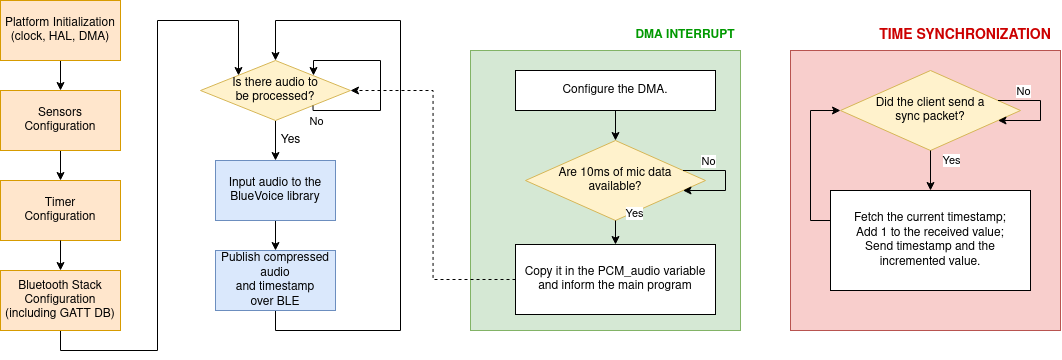
\includegraphics[width=0.85\textwidth]{chap3/figure/BlueVoiceFlow.png}
        \caption{Flowchart of the firmware for the BlueTile that streams audio data.}
        \label{fig:bluevoice-firmware}
    \end{figure}
 
 In this case, the resulting firmware is quite similar to the original one, with the modifications explained in the flowchart in Figure \ref{fig:bluevoice-firmware} and in following list:
 \begin{itemize}
     \item \textbf{Sensor Data Streaming}. I left the data rate of the sensors to the default value (25Hz). There is no necessity to fully disable the functionality from the firmware, because when voice streaming is active, the sensor data streaming is automatically disabled.
     \item \textbf{DMA configuration}. The microphone on the BlueTile board outputs data in the Pulse-Density modulation form (PDM): the frequency of ones is proportional to the sound pressure level. Usually, audio is represented using a different standard, called Pulse-Coded modulation (PCM), composed of 16 bits words ranging from 0 (no pressure) to \(2^{16}\) (maximum pressure). This conversion can be performed in hardware using the Direct Memory Access (DMA) component of the BlueTile SoC, that can asynchronously update the value of a variable (containing audio data) and then inform the main program through an interrupt. Hence, the DMA should be configured in the initialization phase to perform this operation.  
     \item \textbf{Timestamping}. The \textit{BlueVoice} library has been thought to stream audio information in real time, hence there was no need to timestamp the audio data. In my case, as this data is necessary for further analysis, there is the need to provide timestamps along with the audio samples. To do so, I added a GATT characteristic on which timestamping information is published. I also modified one of the \textit{BlueVoice} callback procedures, in particular the \textit{SendData} one, responsible of sending out samples once processed: just before publishing the audio data on its own GATT characteristic, the current timestamp is published on the other one. The client will then join them together.

     I put the implementation of this system in the separated \textit{timestamp\_helper.c} file, that contains the variables (GATT characteristic handle) and the two procedures (GATT characteristic creation, timestamp publishing) necessary for all of this to work.
    \item \textbf{Timer modification}. As done for the other firmware, I disabled the timer that automatically turns off the device after 20 seconds of inactivity if the device is battery-operated.
    \item \textbf{Time synchronization mechanism}. Also in this case, I modified the GATT database to introduce the time synchronization mechanism.
 \end{itemize}
 

\subsection{ST SensorTile.box firmware}
 The SensorTile.box presents some differences from the other device from ST. Even if the software stack is similar, there is no possibility to program the BlueNRG microcontroller, that is controlled by the STM32 Cortex-M4 processor, the only one accessible by the developer. This difference unlocks a great number of other possibilities, thanks to the computing power and the STM32 libraries, but the firmware development becomes a little more complex.
 
 The definitive solution consisted in using the \textit{ALLMEMS-1} firmware example from ST \cite{allmems1}, modifying it according to my needs. In this case, this software has been the best choice, as other ones didn't include support for some sensors like the microphone. It is worth noticing that the SensorTile.box presents no support for the \textit{BlueVoice} library, hence it is possible to extract information from the audio stream, but not to send it real-time to the client. 
 
 Finally, regarding the BLE stack, it is interesting that its abstraction layer is providing C functions working in the same way as they're working in the BlueTile, even if the hardware is quite different. As a consequence, full compatibility with parts of BlueTile firmware is assured: GATT characteristic creation/update, connection configuration, callback procedures all work in the same way. The final firmware is represented in Figure \ref{fig:sensortilebox-firmware}.

      \begin{figure}[ht!]
        \centering
        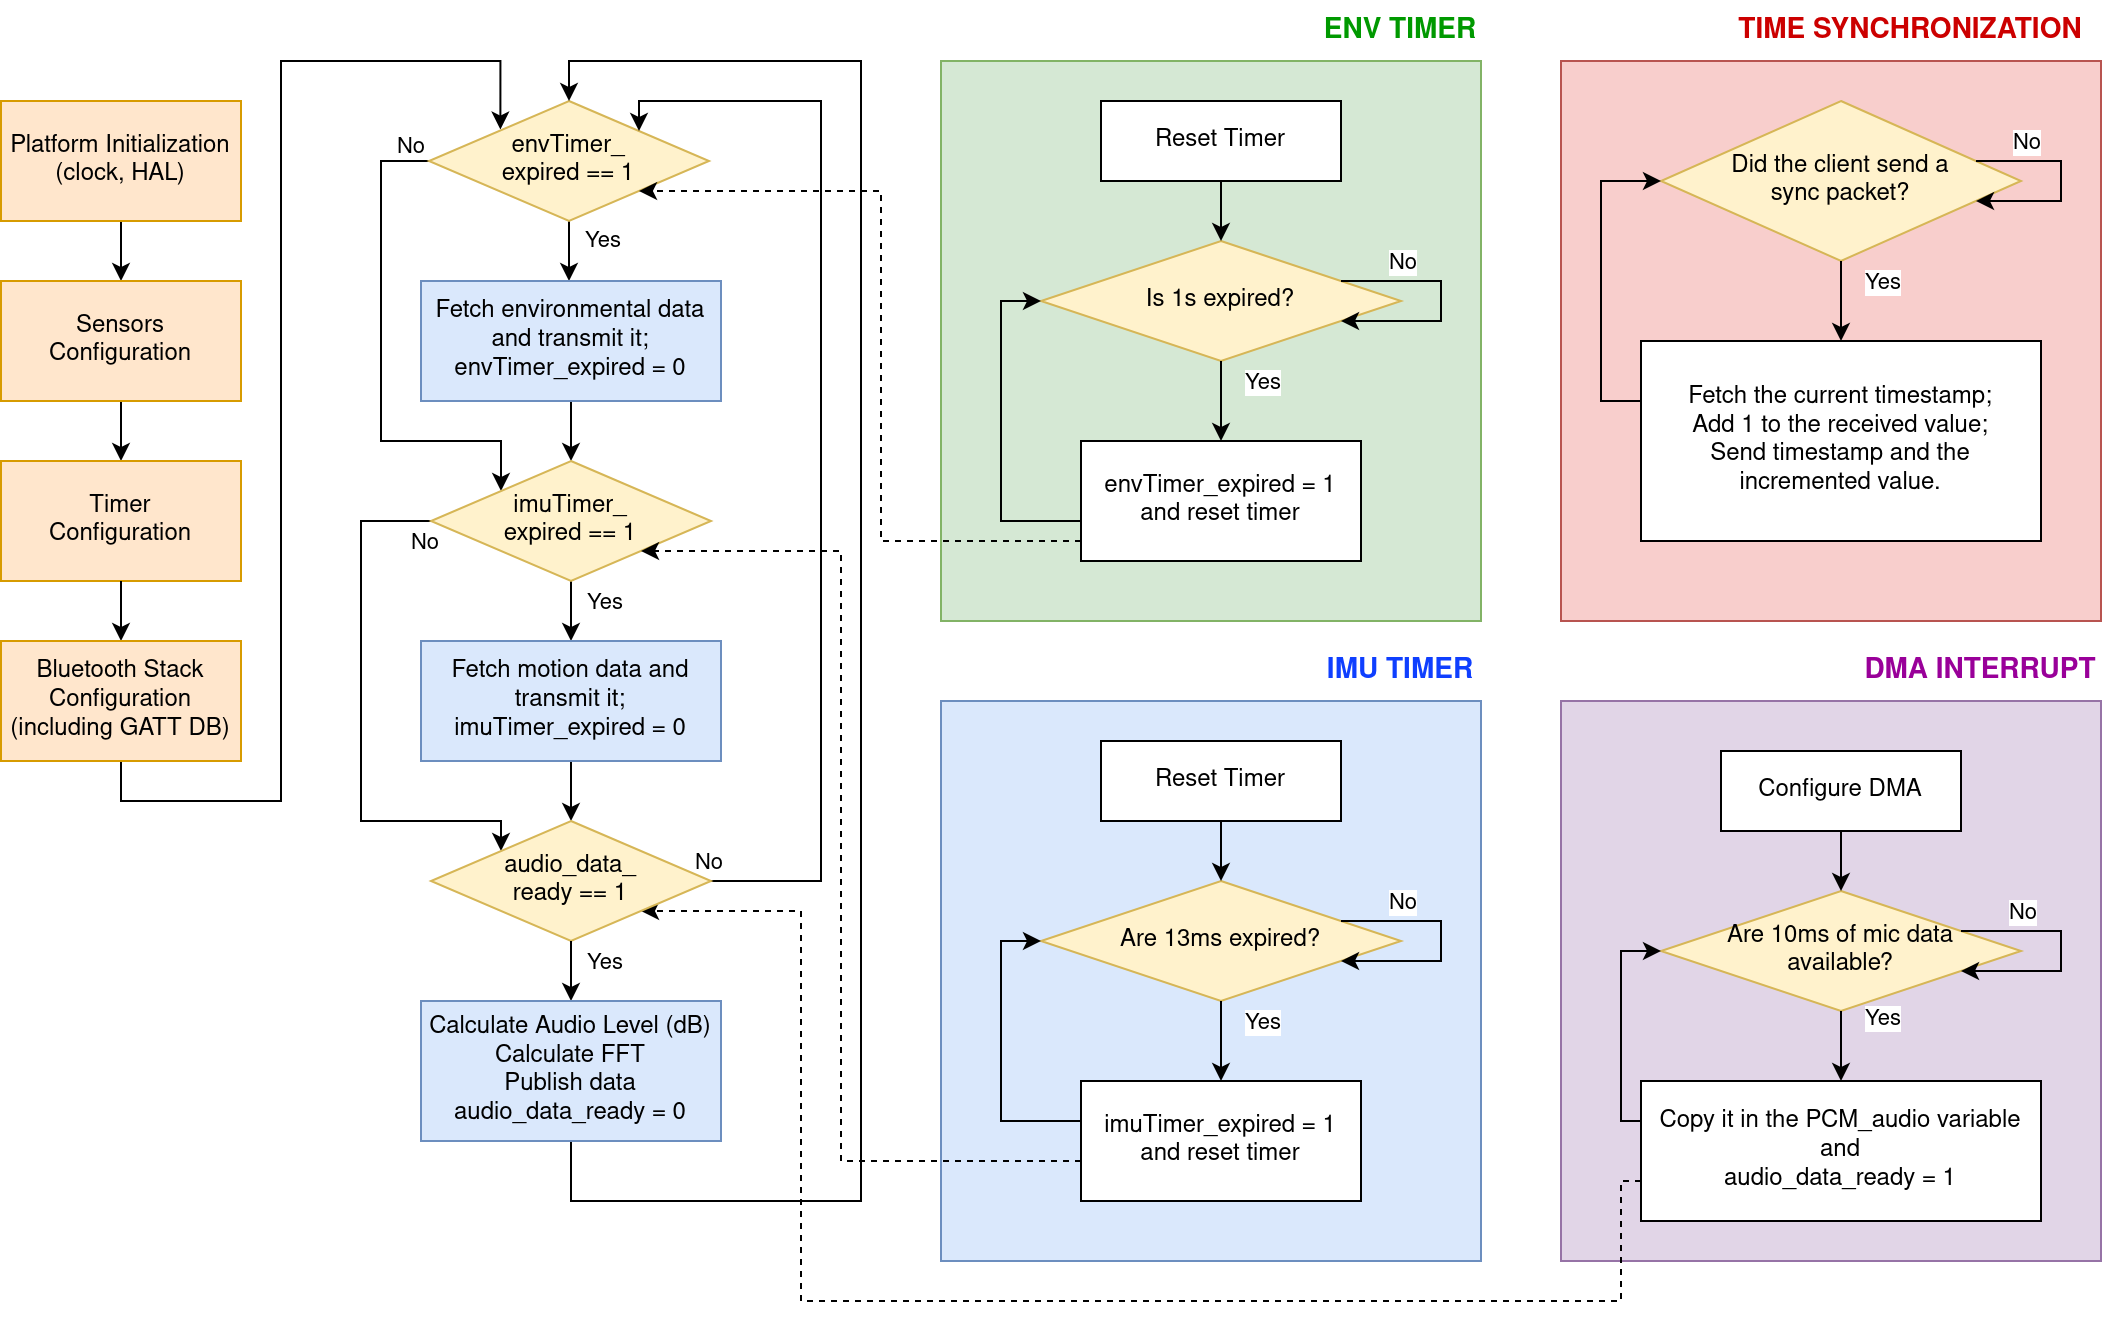
\includegraphics[width=0.85\textwidth]{chap3/figure/STbox.png}
        \caption{Flowchart of the firmware for the SensorTile.box.}
        \label{fig:sensortilebox-firmware}
    \end{figure}

The following list explains the functionalities of the firmware and the work I've done on it:
\begin{itemize}
    \item \textbf{Sensor data streaming}. The information chosen to be transmitted to the client are the IMU (accelerometer, gyroscope, magnetometer), pressure, humidity and temperature sensors. 
    \item \textbf{Data rate modification}. Like what's has been done on the BlueTile, I modified the motion sensors data rate to 75Hz and environmental sensors data rate to 1Hz, setting accordingly the timer variables. 
    \item \textbf{Timestamping}. The timestamping on the SensorTile.box firmware had a different behaviour from the BlueTile one. It would still send the number of milliseconds elapsed from power on, but the three LSBs were shifted out and not sent to the client. To create consistency between devices and add precision (we need time to be as accurate as possible), I disabled the shifting, to transmit the entire timestamp. 
    \item \textbf{Time synchronization mechanism}. Also in this case, I modified the GATT database to make the time synchronization mechanism possible. 
    \item \textbf{Audio processing}. One of the interesting features of the SensorTile.box is the presence of a digital microphone. The ALLMEMS firmware from ST leverages this component offering the streaming of audio level information (in dB). To enrich the details on the surrounding audio, I added the information on the dominant frequency: the samples used to extract the dB information are also input for the \textit{arm\_rfft\_fast\_f32} function from the Common Microcontroller Software Interface Standard (CMSIS) from ARM, that is a a vendor-independent abstraction layer for microcontrollers that are based on ARM Cortex processors. For my use case, it provides an easy way to take advantage of the DSP included in the Cortex-M4 core available on the board. After getting the discrete real Fast Fourier Transform (FFT), the maximum magnitude for each output value is extracted, and the corresponding frequency index is sent on its own GATT characteristic, that I configured before.  
    I would like to underline that, also in this case, the configuration of the DMA has been necessary (as explained in the BlueTile chapter). 
    \item \textbf{Removing undesired functionalities}. The ALLMEMS firmware contains a lot of libraries from ST, used for sensor fusion and feature extraction (activity, gesture, position recognition and so on). To save battery, space and computational power (the FFT operation is pretty intensive), I disabled all these functionalities by commenting out their initialization code lines, along with the relative callback functions.  
\end{itemize}


\section{The Time Synchronization Mechanism}
One of the most challenging parts of this thesis has been the development of a time synchronization mechanism for the ST devices, as MetaMotion ones already embed their own closed-source implementation. Three main issues should be overcome to do so: first of all, the limited computational power available on the sensor nodes (in particular, the BlueTile ones), the need to implement this system at the higher application layer of the BLE stack (as lower levels are not accessible by the developers), and the need for a compromise between time accuracy and high data rates. 

The main idea is to leverage on the client, that is a Linux computer running a Python script and a fundamental part of our sensors system. It can be used to provide a reference clock for all the data coming from the sensor nodes. To reduce the number of exchanged packets, an application similar to the receiver-to-receiver one could be used, in which a reference broadcasts messages simultaneously to all devices, and then they can use their reception timestamps to synchronize.  

In particular, the system I implemented consists in the client sending packets to all devices at regular intervals, using the \textit{WRITE\_NO\_RESPONSE} property of a GATT characteristic specifically created for this scope on the sensor nodes. That particular property is the fastest way to send data to a BLE device, as no response is necessary and only one packet is sent. As soon as the remote device receives the packet, the relative callback procedure is automatically called by the BLE stack of the node: in that function, the packet is sent back with its original content (a number) incremented by one, and the internal timestamp. 

The client will then receive that information, and associate the received timestamp to the current Unix epoch time expressed in milliseconds using the \textit{time} library of Python 3.10, which returns a precise value (while previous versions of Python weren't able to do so). Then, the successive samples will be timestamped using the available information: 1) the UNIX time obtained in the resynchronization moment \(t_{UNIX}\), 2) the timestamp of the resynchronization moment \(t_R\) and 3) the device timestamp of the sample under analysis. \(t_S\). The result is calculated with Equation \ref{timestamp-formula}.
\begin{equation} \label{timestamp-formula}
T = t_{UNIX} + (t_S - t_R) 
\end{equation}

The resynchronization procedure can be executed at any desired interval by simply modifying the value in the Python script of the client. In the experiments explained in this thesis, the interval is set to 1s, which was able to give good performances when keeping a data rate of 75~Hz. More details in the Results section. 
\section{Client for ST devices}
The client for the ST sensor board is a Python script for Linux hosts that handles connection, data collection and time synchronization with all the sensor boards from ST. Of course, the client is compatible with the firmware that has been developed for this thesis only, as the time synchronization and other details do not follow any existing standard.

I'm reporting more details on the client structure and behaviour in the following list and flowchart (Figure \ref{fig:st-client}). 

     \begin{figure}[ht!]
        \centering
        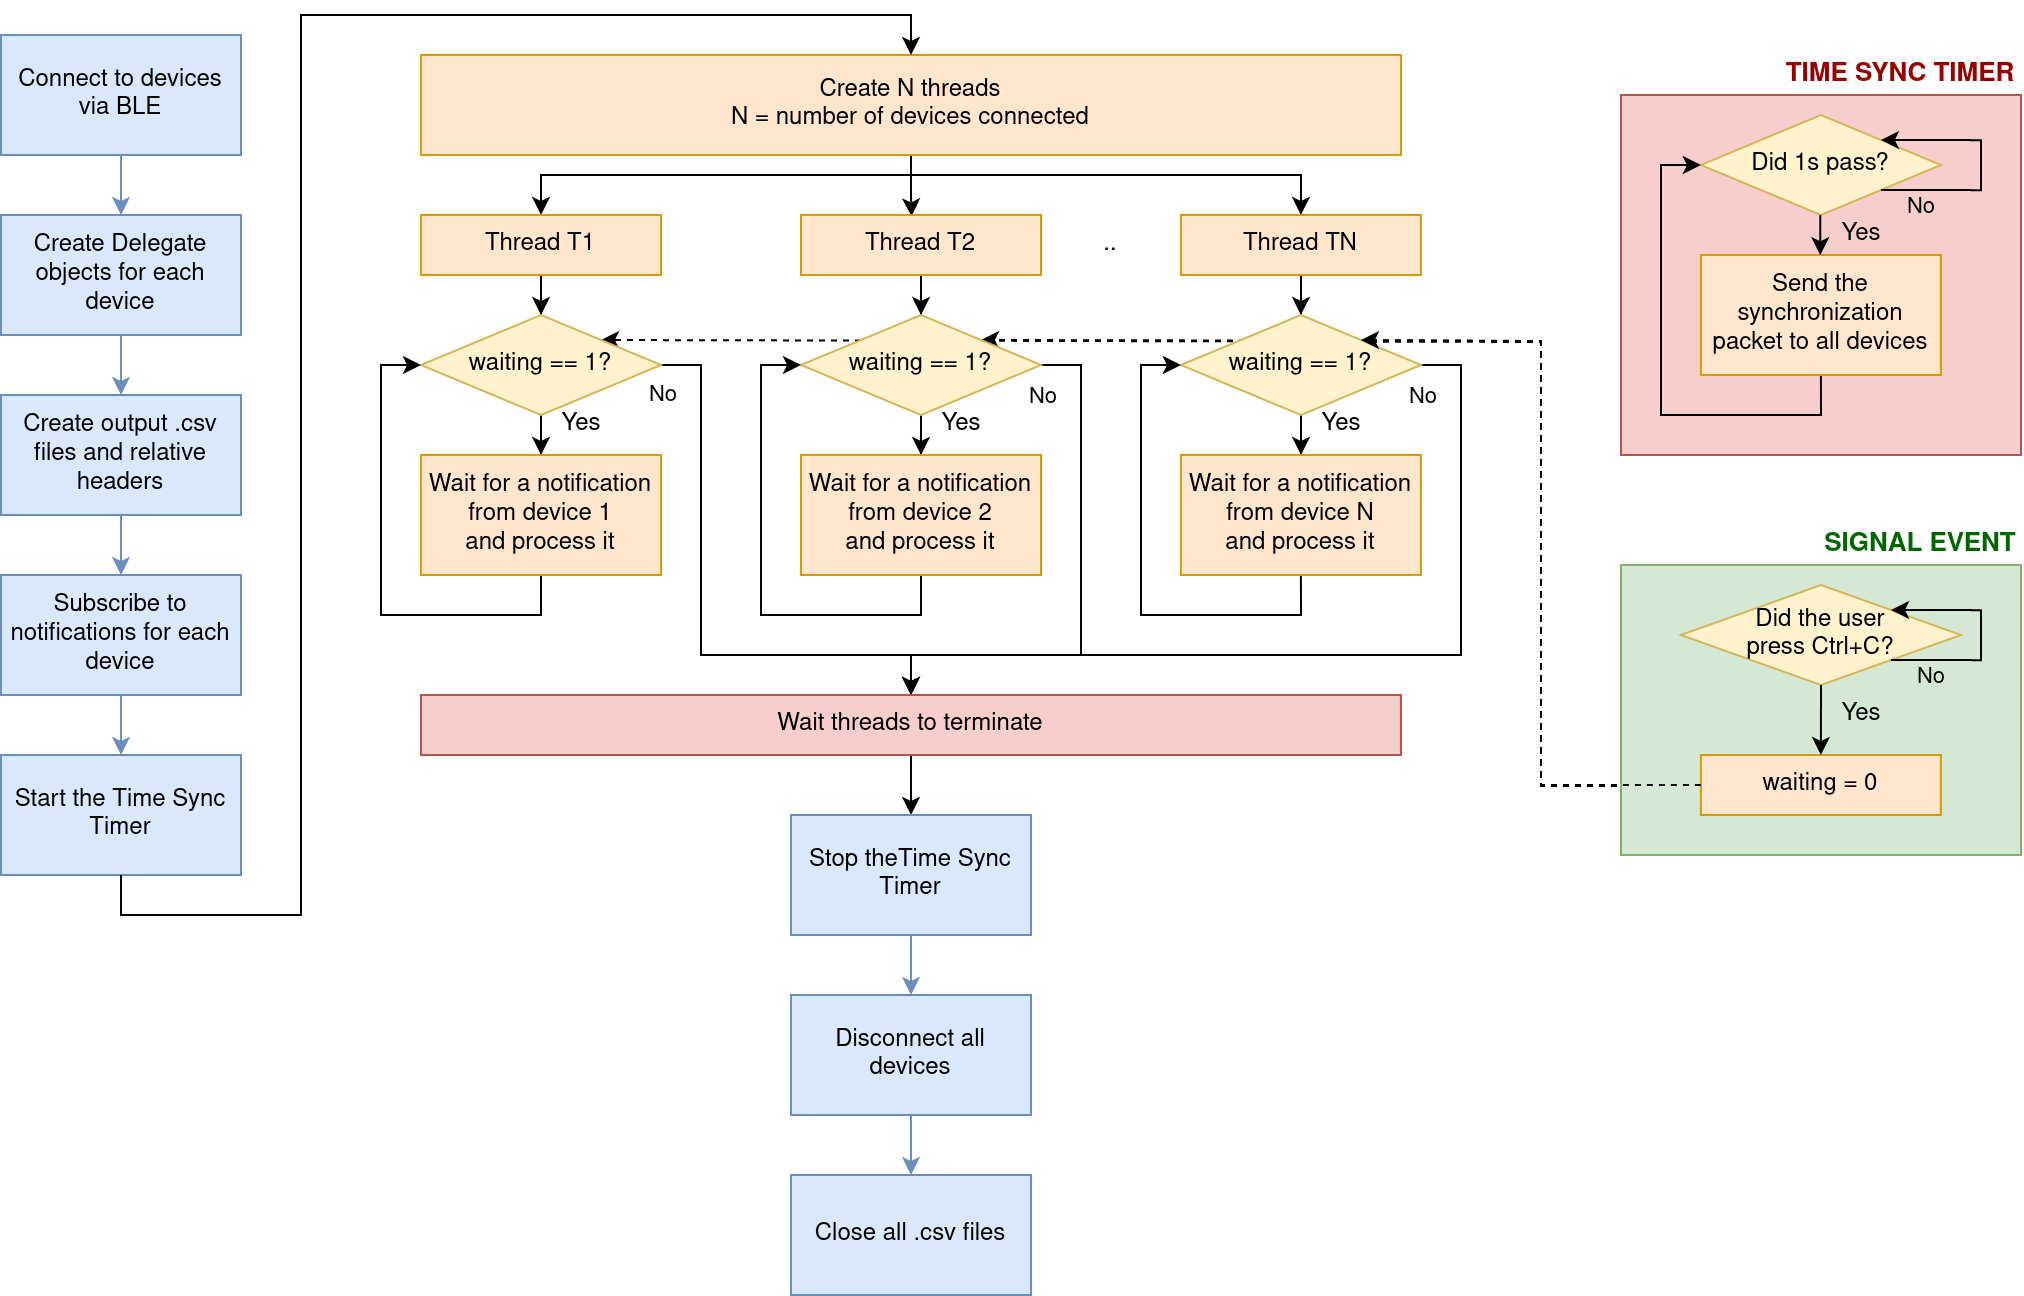
\includegraphics[width=0.85\textwidth]{chap3/figure/Flowchart_st_client(1).png}
        \caption{Flowchart of the client for ST sensor nodes.}
        \label{fig:st-client}
    \end{figure}

\begin{itemize}
    \item \textbf{Connection}. In the first part of the script, I used the \textit{BluePy} library for Python to perform connection to all of the devices. All the information necessary for the connection are reported in a list of dictionaries, each one presenting a) the device name, b) the device MAC address, c) the device type and d) the interface to use for connection. The device type is necessary for the client to understand which features are available (for example, audio dominant frequency is available for the SensorTile.box, only). Also the interface is quite important for our use case, because using multiple Bluetooth adapters leads to better performances (more details in the Results part). It is possible to connect to multiple devices using only one client.

    Once the connection to a device is performed, an object, inherited from the BluePy library, is created for each device. It is called a Delegate, and it contains information for the connection to that device: it is fundamental in our environment, where more than one device is connected. In particular, in this implementation the Delegate holds a) the name of the device; b) the handles used to recognize the type of received data (IMU, environmental, time, audio...) c) the file handles, to write the data into, d) the procedure to be called each time data is received from the device. 

    \item \textbf{Notification handling}. As soon as connection is performed and all Delegates are ready, the clients \textit{subscribes} to the GATT characteristics it is interested to. This procedure varies, based on the type of the device the client it's working with. For example, in the case of the BlueTile (sensing firmware), the client subscribes to IMU sensors, environmental sensors and time synchronization characteristics. 

    After the subscription, each time the sensor node sends data on a particular characteristic, the \textit{handle\_notification} function of the Delegate is called. It will compare the handle with the ones saved in it, understand the type of data received and behave accordingly: in case of sensor data, it is further processed (to use consistent measurement units with MBIENTLAB devices) and written to file, while if it is time synchronization data, the received timestamp and the immediate Unix epoch are saved in the Delegate and used to process successive packets. 

    It is important to add that the BluePy library makes use of the \\\textit{wait\_for\_notification} blocking function, that waits for notification from the precise device it is called from. As we are dealing with more than one device, it is necessary to create different threads, one per node, and then call the function in them using a while condition. As soon as the while condition becomes false, the thread will terminate. 

    \item \textbf{BlueVoice data handling}. In case the ST client is connected to a device of type \textit{bluevoice} (i.e. a BlueTile with the audio streaming firmware), the behaviour is the same of the other ones, but the data received from the node is (of course) treated differently. 
    
    First, timestamps are received from a different GATT characteristics, and should be joined to the audio samples packet. This is performed by using FIFOs lists for both data. 

    Second, data is received compressed, using the ADPCM codec. It means that 16B samples are reduced to 4B samples, that contains only the differences from the previous set of samples. As some packets may get lost, the reconstruction process may not work on the long period: to solve this, the BlueVoice library also sends the so-called sync packets (at lower frequencies). Those contain uncompressed data on which the difference packets can be applied to reconstruct the original signal even if some segment went lost. 
    All this information is processed inside the corresponding functions, \textit{process\_sync} and \textit{process\_audio}, that are released by ST in their GitHub account. 

    \item \textbf{Time Synchronization}. After completing the subscription to all GATT characteristics, the so-called \textit{Repeated Timer} it is created. It is a small Python module making use of the \textit{time} and \textit{threading} libraries to generate a timer that fires at defined intervals, executing a defined function. It is important to note that it has been designed to consider the real interval between firings: the time needed to perform the instructions inside the function will not count. 

    In my implementation, one timer is configured to be fired each second: in the procedure, the synchronization packet is sent to all devices. As explained in Section 3.2, those will respond with a notification, that will be managed accordingly. Other firing intervals can be configured, but smaller ones cause bigger number of packets to be elaborated and exchanged: 1~s is the best tradeoff I found between the number of lost packet and the synchronization accuracy, while 0.5~s caused big percentages of packet loss. 

    \item \textbf{Program termination}. The Ctrl+C signal has been configured to call a procedure that will change the value of the \textit{waiting} variable. That variable is the one that keeps the notification waiting threads alive. In this way, the threads can terminate and join to the main program, that will disconnect from all nodes, close the files and terminate. 

    \item \textbf{BluePy modification}. The BluePy library suffers from a bug that generates exceptions if a GATT characteristic is written while there are multiple threads waiting for notifications. In particular, an object indicating the correct transmission of the packet should be returned to the \textit{writeToCharacteristic} function, that will terminate afterwards. Sometimes that object is received by one of the \textit{wait\_for\_notification} procedures, that are not expecting it, generating an exception. To resolve it, I implemented a workaround, consisting of a) making \textit{wait\_for\_notification} ignore that particular object when received and b) forcing \textit{writeToCharacteristic} to return without waiting for the confirmation object. This does not seem to cause problems in the resynchronization procedure, and we can be confident that the packet is sent by the BLE stack without the need for confirmation. Anyway, this should be considered as only a workaround,  because the problem should be resolved by re-thinking this part of the library (confirmation of the successful transmission is quite important in any case). 
\end{itemize}

\section{Client for MBIENTLAB devices}
I found writing the client for MBIENTLAB MetaMotionS much simpler, as the available APIs and examples are easy to understand and implement. There is no need to implement any time synchronization mechanism, as it's already available by default. Starting from the available Python example, available from the vendor's Github page \cite{metawearsdk}, that is performing the streaming of accelerometer data, I wrote the final version of the script with the following features, with the flowchart represented in Figure \ref{fig:meta-client}.

     \begin{figure}[ht!]
        \centering
        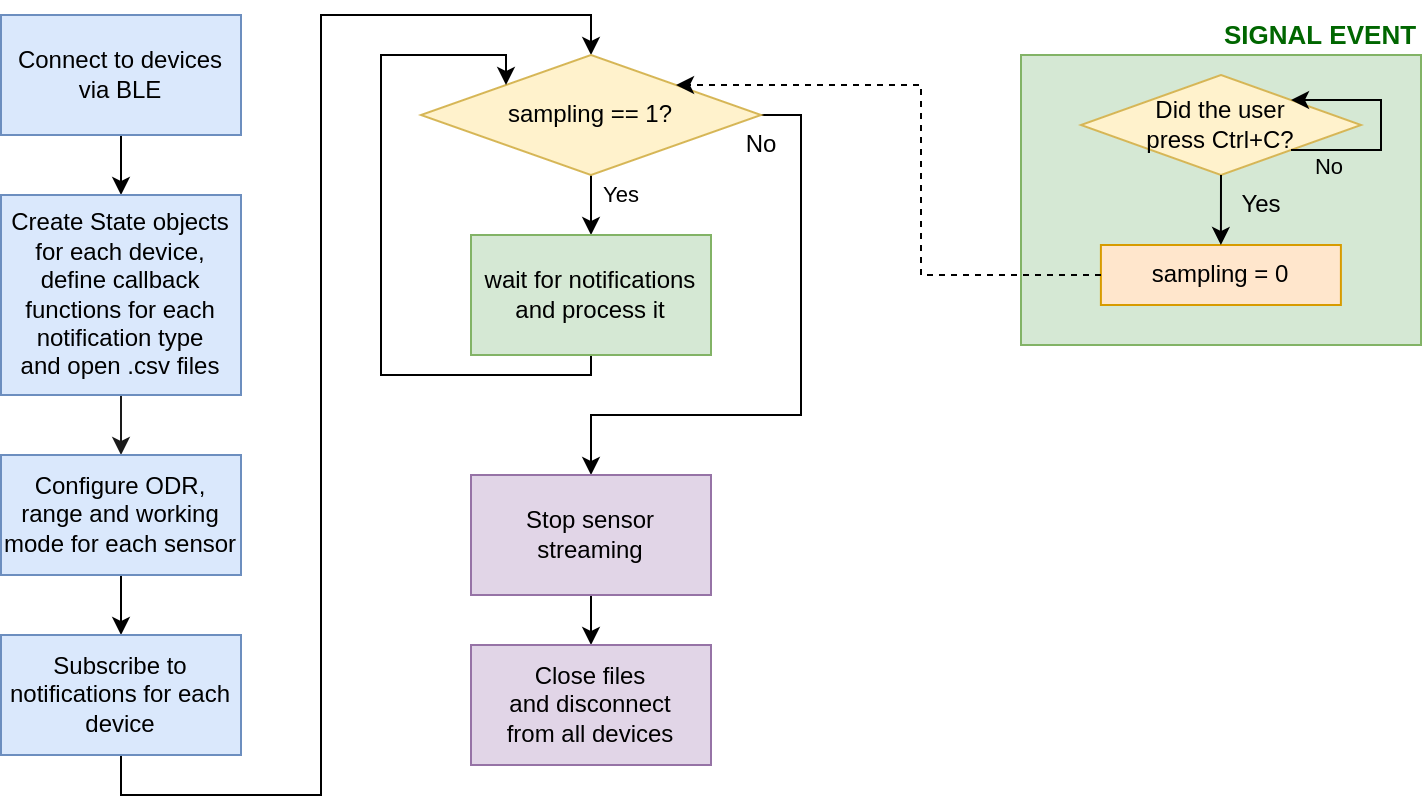
\includegraphics[width=0.85\textwidth]{chap3/figure/Flowchart_meta_client.png}
        \caption{Flowchart of the client for MBIENTLAB sensor nodes.}
        \label{fig:meta-client}
    \end{figure}


\begin{itemize} 
    \item \textbf{Connection}. Also this script support the connection to multiple devices, represented in a list of dictionaries, using multiple Bluetooth adapters. For each sensor node, it is reported a) a name, b) the MAC address of the device and c) the MAC address of the interface to use for connection. The connection is performed by the APIs, so no need to use BluePy (or similar libraries). 

    After the connection, similar to the script for ST nodes, a set of objects, called States, is created. Each of them is responsible for one device, and contains a) the device name, b) the pointers to the functions to be called when data is received and c) the handles of the files in which data is stored.

    The functions are used to take the data from the received packets and save it inside .csv files correctly formatted. To do so, the function \textit{parse\_data}, from the MBIENTLAB APIs is used to get a string containing all data: a regular expression will extract the interesting values from the string and write them into the file. 
    \item \textbf{Configuration}. In the configuration phase, each sensor is configured in its ODR (Output Data Rate), power mode (low power or high accuracy and so on) and range. The sensors configured are IMU (accelerometer, gyroscope, magnetometer), temperature and pressure. This procedure is repeated for each sensor node. At the end, the data collection is started.
    \item \textbf{Data collection stop}. To perform the data collection, I used the Python \textit{sleep} function to make the client wait for notifications. Of course, in the meantime all the received data is processed by the functions pointed inside the State objects. The sleep function, configured to wait for 1s, is repeated until the \textit{sampling} variable remains True: as soon as the Ctrl+C signal makes it become False, the sleep will not be repeated and the Python script will continue its execution. The last lines of code will stop the sampling, reset the sensors, close all the files and print a sum up of the received information. 
\end{itemize}

\section{MATLAB data extraction scripts}
Thanks to the ton of already available libraries and functions for data processing, MATLAB has been the first choice when dealing with the elaboration of all the sensor information retrieved from the data collection campaigns. Transforming CSV values into MATLAB data structure is immediate (the \textit{readtable} function is enough), and then the Signal Analysis Toolbox contains an extensive set of tools to work on those values with ease. In particular, I prepared the following scripts:
\begin{itemize} 
    \item \textbf{Data Extraction for ST devices}: works with Acceleration, Gyroscope and Magnetometer data. It reads all the values, and plots them over time using the MATLAB plotting feature. Then, all the data is modified for the Signal Analyzer application: the timesync set of values is transformed into a square wave, to represent the moments in which the re-synchronization happens, then all the signals are coupled with their timestamp generating \textit{timeseries} data structures. Those timeseries are further analyzed, to order them in the time domain and remove duplicates. In this way, the signals are ready to be shown and elaborated with MATLAB toolboxes.
    \item \textbf{Data Extraction for Meta devices}: it behaves like the one for ST devices, but takes into account the slight differences of CSV data generated by the MBIENTLAB ones. Then, everything remains the same: plots are shown, \textit{timeseries} are generated and elaborated. In particular, the timeseries variables have been called in a different way, in order for them to be distinguished from the ST ones.
    \item \textbf{Data Extract for Voice}: the goal of this script is to reconstruct the audio signal from the CSV file generated by the BlueTile with BlueVoice enabled. As the timestamping mechanism is not as precise as the one used for sensor data (due to the closed-source BlueVoice library), only the timestamps generated at resynchronization events are used, and all the samples in the middle receive regularly intervalled timestamps between the two events. Reducing the re-synchronization interval could be advantageous in this case, but the number of packet loss could be higher, making the audio quality sensibly lower. Also in this case \textit{timeseries} structures are created and elaborated to be shown afterwards in the Signal Analyzed application.
    \item \textbf{Data Extract for Frequencies}: it works only with the frequencies in the CSV generated by the SensorTile.box device. It behaves like the acceleration/gyroscope script, but works with frequencies, that are transformed from the indexes between 0-128 into the real frequencies values, and then scaled by a factor of 1000: this is necessary to make them show in the same plot of the acceleration values, for example. Also in this case, everything is modified to be shown correctly in the Signal Analyzer application. 
\end{itemize}

\section{Calibration Script}

An important step when dealing with accelerometer and gyroscope data is taking care of axes alignment. For example, if the application involves installation of the sensors system on a car, it is important for the boards to be positioned in a coherent way: all the sensor chips have their own axes orientation, and it's a good idea to align them to the vehicle ones. 

A problem may arise if the final user puts the sensors in a wrong way, rotated with respect to the desired direction. In this case, the obtained data should be post-processed accordingly, to get reasonable results: in particular, a rotation matrix should be calculated and then multiplied to the raw acceleration data. 



I had at my disposal an algorithm, wirtten for MATLAB, able to calculate the roll, pitch and yaw angles, developed by the research group I'm working with for this thesis (Electronic Design Automation Group) and optimized for embedded systems application: this algorithm iterates over GPS and IMU data, performing two kinds of calibration, explained as follows.
\begin{itemize}
    \item \textbf{Static Calibration}. Working on a subset of samples, the available data is analyzed to verify if the vehicle the sensor is mounted on is static. If this is the case, the subset of samples is passed to a dedicated procedure able to extract two angles: alpha (roll) and gamma (pitch). 
    \item \textbf{Dynamic Calibration}. Also in this case a subset of samples is analyzed, but here the algorithm verifies if the vehicle is proceeding in a straight path. This step is necessary because, if that condition is met, the buffer of samples undergoing this condition is elaborated, along with the alpha and gamma angles: the output is the beta (yaw) angle. 
\end{itemize}

Once the three angles have been calculated, it is possible to generate the three rotation matrices to be applied to the motion data \(m_{\alpha} , m_{\beta} , m_{\gamma}\) as represented in Equations \ref{m-alpha}, \ref{m-beta} and \ref{m-gamma}. The goal, given the reference system \(R_S\) of the IMU sensors, is to achieve the alignment with the reference system \(R_M\) of the vehicle, as explained in Figure \ref{fig:reference-systems}.

    \begin{figure}[ht!]
        \centering
        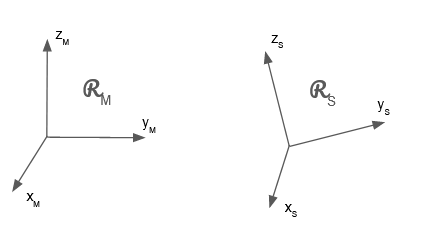
\includegraphics[width=0.5\textwidth]{chap3/figure/calibration_algo_axes.png}
        \caption{Example of sensors reference system compared to vehicle reference system. }
        \label{fig:reference-systems}
    \end{figure}

\begin{equation} \label{m-alpha}
m_{\alpha} = \begin{bmatrix}
    cos(\alpha)     & 0     & sin(\alpha)       \\
    0               & 1     & 0                 \\
    -sin(\alpha)    & 0     & cos(\alpha)       \\
\end{bmatrix}
\end{equation}


\begin{equation} \label{m-beta}
m_{\beta} = \begin{bmatrix}
    cos(\beta)      & -sin(\beta)     & 0       \\
    sin(\beta)      & cos(\beta)      & 0       \\
    0               & 0               & 1       \\
\end{bmatrix}
\end{equation}

\begin{equation} \label{m-gamma}
m_{\gamma} = \begin{bmatrix}
    1      & 0     & 0       \\
    0      & cos(\gamma)      & -sin(\gamma)       \\
    0               & sin(\gamma)               & cos(\gamma)      \\
\end{bmatrix}
\end{equation}

The system I'm working on does not include any GPS sensor, hence this algorithm required some modifications in order to be useful. In particular, I modified the two functions that are responsible of recognizing the static and dynamic conditions, generating the corresponding sample subsets. In the new version of the script, these functions are no more accepting GPS data as inputs, and they verify (a) the static condition by checking if the variance of both acceleration and gyroscope samples is below a certain threshold and (b) the dynamic condition by calculating the variance of the gyroscope samples and comparing it to a threshold. Then, the calculation of the angles remains as before, because that step requires the IMU samples only. Some work was necessary to correctly fix the thresholds for the variance values, that have been decreased from the original values to reach more precise results in calibration. 

In Figure \ref{fig:calibration-flow} the flowchart of the algorithm is reported. The two different kind of calibration are reported in different colors. 

It is evident that the calibration is performed in an iterative way, by repeating the static and dynamic calibration over different chunks of samples (moving the \textit{start} index). Each cycle will generate different values for the angles, and at the end the median value is calculated and shown as output.
The two calibration procedures will take the sample corresponding to the \textit{start} index, and then add values (one second of samples per cycle) until the variance of the buffer overcomes the threshold value. In this case, the last second of samples is flushed (because the condition is no more met), and, if the remaining ones represent the static/dynamic condition for at least a certain number of seconds, those IMU samples are used to perform calculation of the required angles (alpha and gamma for static, beta for dynamic). 

    \begin{figure}[ht!]
        \centering
        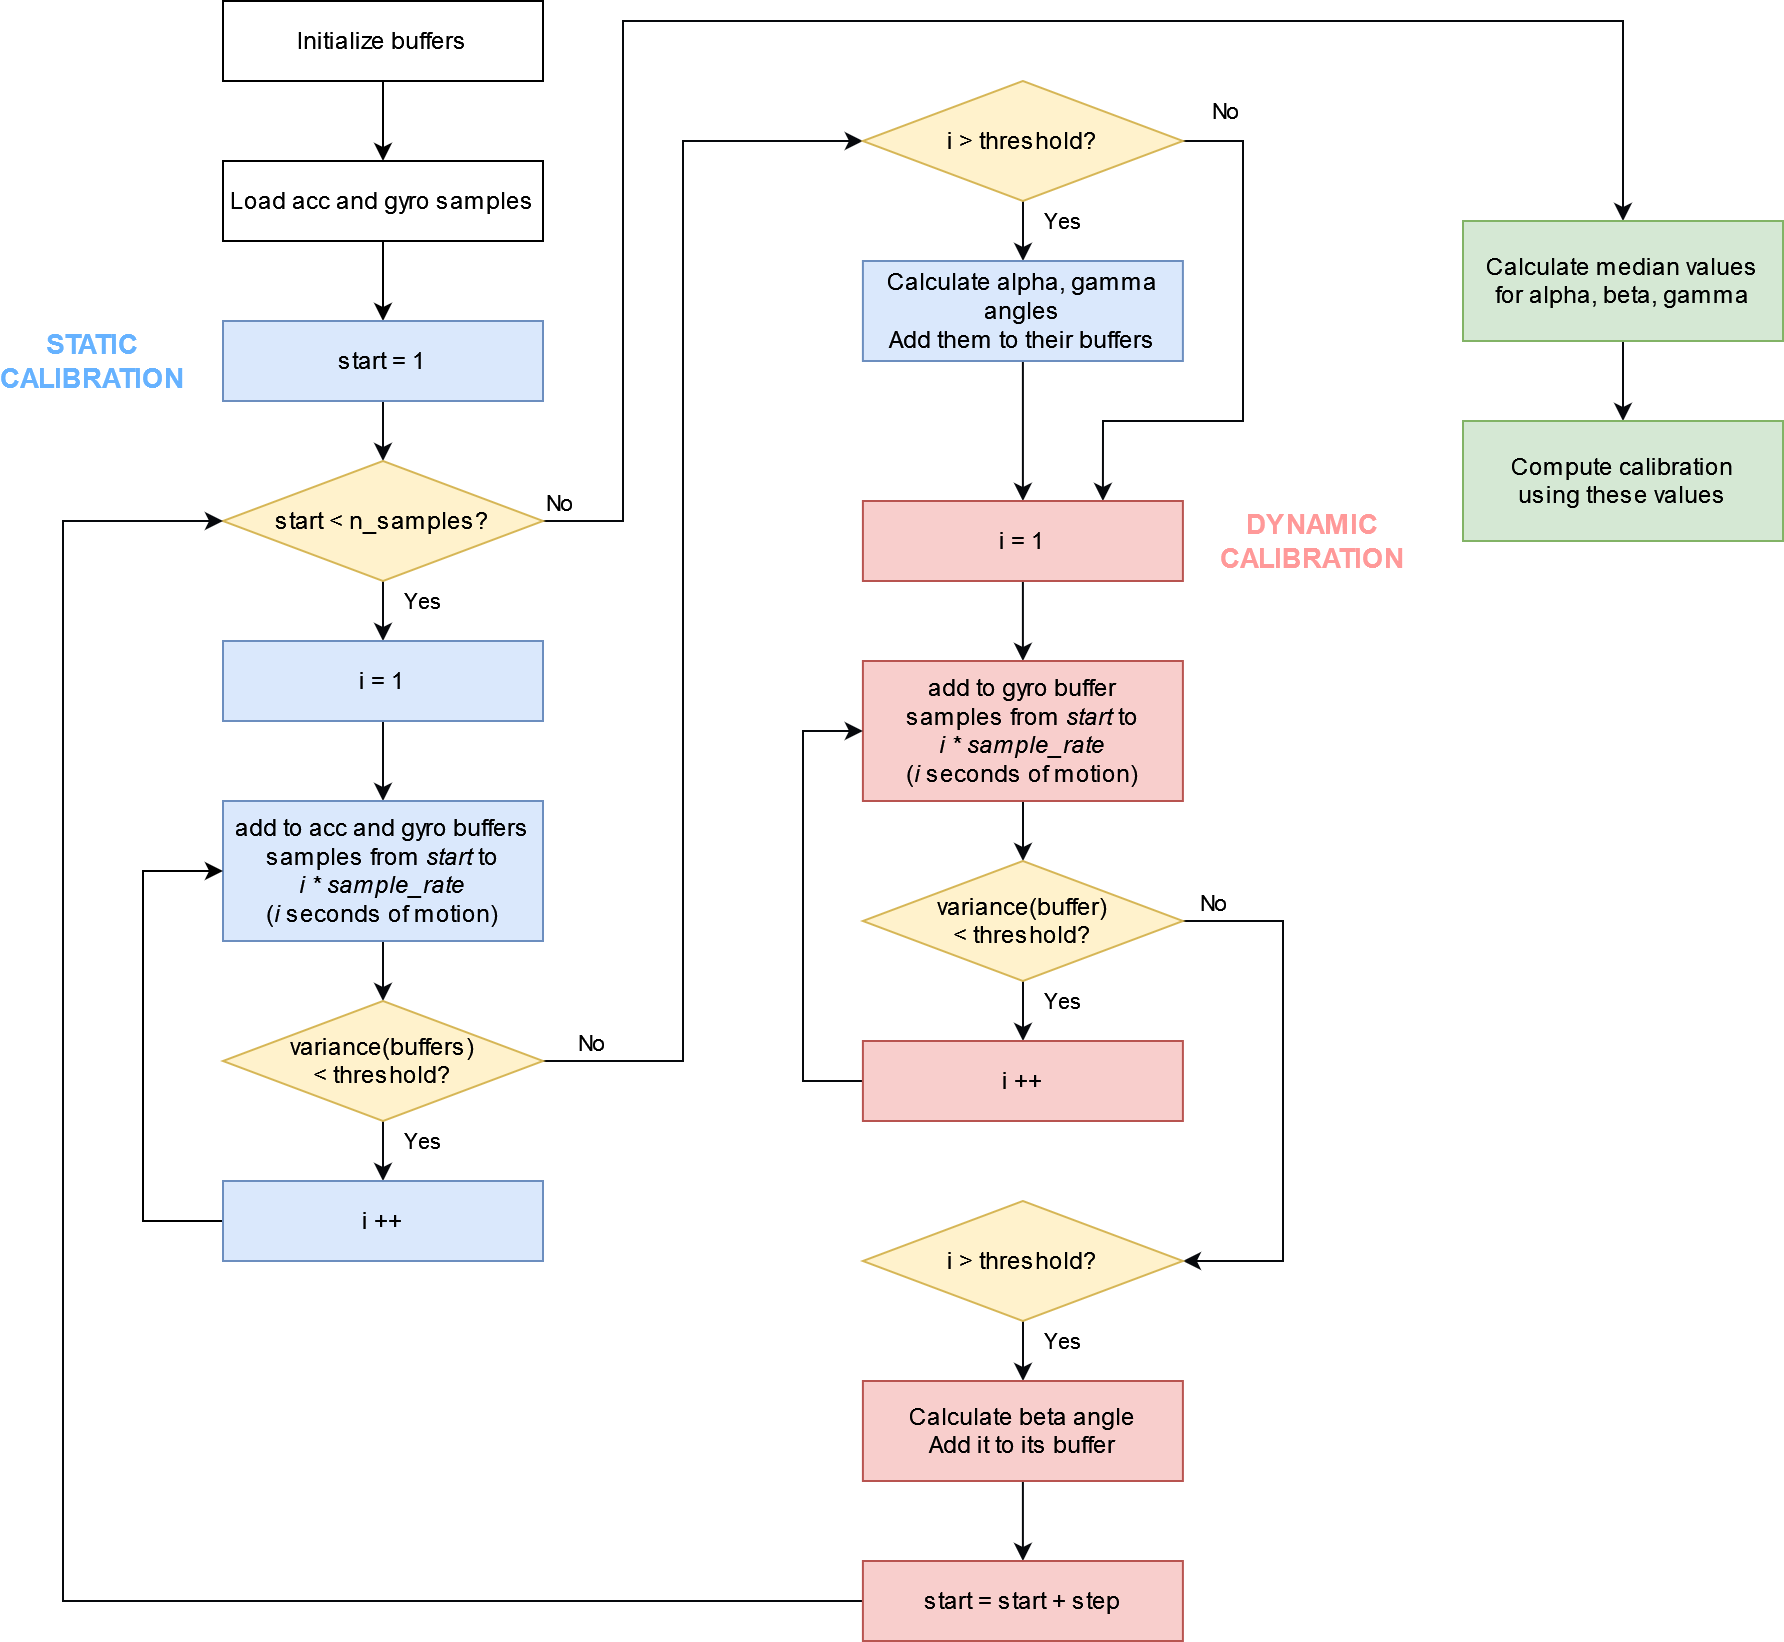
\includegraphics[width=\textwidth]{chap3/figure/calibration_flowchart.png}
        \caption{Flowchart of the script that perform calibration of the axes.}
        \label{fig:calibration-flow}
    \end{figure}

\clearpage
\section{Used tools}


\subsection{Agno Framework}

Agno is an open-source, Python-based agentic framework designed to facilitate the development of intelligent AI agents with integrated memory, knowledge, tools, and reasoning capabilities. Agno provides a lightweight, composable architecture that emphasizes declarative agent construction, model-agnostic design, and first-class tool support. The framework enables rapid prototyping and deployment of multi-agent systems through a clean API that abstracts the complexities of agent orchestration, tool coordination, and state management while maintaining full transparency for debugging and auditability.


\subsubsection{Tool System and Toolkits}

Tools occupy a central role in Agno's architecture as primary mechanisms for agent interaction with external systems. Tools are Python functions or classes that expose specific capabilities to agents, enabling interaction with external systems such as APIs, databases, web search engines, and file systems. The framework provides two primary tool abstractions: individual \textbf{function tools} for single operations and \textbf{toolkits} for collections of related functions that share internal state and coordinate behavior. Toolkits are implemented as Python classes that register multiple methods as callable tools, allowing agents to invoke them transparently based on task requirements.

\subsubsection{RAG Tools for Information Retrieval}

In the thesis implementation, four core toolkits from Agno's pre-built collection specifically utilized, to enable comprehensive information retrieval across web and academic sources:

\textbf{TavilyTools:} Provides advanced web search capabilities through the Tavily API, a search engine optimized for LLM-driven applications. The toolkit supports configurable search depth (\texttt{standard} vs.\ \texttt{deep}), maximum token limits per result, and output formatting (sourcedAnswer for synthesized responses with citations vs.\ searchResults for raw context data). TavilyTools was employed in the web research branch to execute primary web searches with advanced depth settings, retrieving up to 5 documents per query with full raw content preserved for subsequent LLM-based parsing and summarization.

\textbf{ArxivTools:} Enables retrieval of academic preprints and research papers from the arXiv repository. The toolkit queries the arXiv API using structured search parameters and returns paper metadata including titles, authors, abstracts, publication dates, and arXiv identifiers. ArxivTools was integrated into the academic research branch to complement web-based sources with peer-reviewed and domain-specific scientific literature, ensuring coverage of cutting-edge research findings and formal scholarly discourse.

\textbf{DuckDuckGoTools:} Provides privacy-focused web search through the DuckDuckGo API, serving as a fallback search backend when Tavily or other primary tools are unavailable or rate-limited. The toolkit executes keyword-based searches and returns result snippets, titles, and URLs. While not the primary search tool in the implementation, DuckDuckGoTools was configured as an alternative within the agent toolkit stack to ensure search robustness and redundancy.

\textbf{GoogleSearchTools:} Enables search through Google's Custom Search Engine API, providing access to indexable web content with support for configurable result limits and ranking. The toolkit returns structured results including titles, snippets, and URLs. GoogleSearchTools serves as an alternative search provider within the agent toolkit stack, offering broader web coverage and integration with Google's search index while being subject to rate limits and quota constraints.

\subsubsection{Agent Execution and Tool Coordination}

LangGraph gents execute tools through an internal reasoning loop that analyzes user queries, determines which tools are necessary, invokes them sequentially or in parallel, and synthesizes their outputs into coherent responses. Tool calls are transparent by default (configurable via \texttt{show\_tool\_calls}), enabling inspection of agent decision-making and facilitating debugging. In my implementation, agents were instantiated with the Ollama backend and configured with specific toolkits based on branch requirements (TavilyTools for web research, ArxivTools for academic research).

\subsubsection{Integration of Agno Tools into LangGraph Workflows}

Agno tools integrate seamlessly into LangGraph state machines as callable functions within graph-based workflows. In the developed architecture, each research branch (web and academic) instantiates branch-specific toolkits, executes queries through the tool coordination layer, and returns raw search results to the LangGraph state for subsequent parsing, deduplication, and summarization. This integration pattern leverages Agno's composable tool abstractions while maintaining LangGraph's control over overall workflow orchestration, state management, and conditional routing.




\subsection{DeepEval}

DeepEval is an open-source, LLM-powered evaluation framework designed to assess the quality of RAG systems through quantitative, interpretable metrics. Rather than relying on manual evaluation or subjective criteria, DeepEval employs the LLM-as-a-judge paradigm, where a language model autonomously evaluates generated outputs against multiple complementary dimensions. This systematic approach enables comprehensive quality assurance of generated content without human annotation.

\subsubsection{Core RAG Evaluation Metrics}

DeepEval provides four fundamental built-in metrics specifically designed for RAG pipeline evaluation:

\textbf{Faithfulness:} Measures whether the generated output's claims are factually grounded in the retrieved documents. Faithfulness answers: \textit{What fraction of the generated statements are supported by the retrieval context?} This metric prevents hallucination, the generation of information not present in sources, by validating each factual claim against provided documents. Formally:

\begin{equation}
\text{Faithfulness} = \frac{\text{Supported Claims}}{\text{Total Claims}}
\end{equation}

\textbf{Answer Relevancy:} Evaluates whether the generated output directly addresses the user's original query. Answer relevancy measures topical alignment by classifying generated statements as relevant or tangential to the research question. This metric ensures the output focuses on answering what was asked, independent of factual correctness. Formally:

\begin{equation}
\text{Answer Relevancy} = \frac{\text{Relevant Statements}}{\text{Total Statements}}
\end{equation}

\textbf{Contextual Relevancy:} Assesses the quality of retrieved documents by measuring whether they are genuinely relevant to the user's query. Unlike faithfulness, which validates the generator's use of context, contextual relevancy validates the retriever's selection process. This metric identifies whether the retrieval system has selected appropriate source documents. Formally:

\begin{equation}
\text{Contextual Relevancy} = \frac{\text{Relevant Retrieval Documents}}{\text{Total Retrieved Documents}}
\end{equation}

\textbf{Hallucination Detection:} Explicitly identifies claims in the generated output that contradict or lack support in the retrieval context. This metric flags negative cases, statements that directly contradict sources or introduce unsupported assertions, distinct from positive alignment measured by faithfulness. Formally:

\begin{equation}
\text{Hallucination Score} = 1.0 - \frac{\text{Contradicted/Unsupported Claims}}{\text{Total Claims}}
\end{equation}

\subsubsection{Metric Scoring and Threshold-Based Evaluation}

Each metric produces a score in the range \([0.0, 1.0]\), where 1.0 represents perfect performance and 0.0 represents complete failure. The interpretation of metric scores typically employs a threshold-based approach: scores above a defined threshold are considered acceptable, while scores below the threshold indicate quality concerns requiring investigation or remediation.

The threshold selection is a design choice that reflects the acceptable quality level for the application. In academic or high-stakes applications, thresholds may be set higher (e.g., 0.70, 0.75) to ensure maximum reliability. In exploratory or low-stakes scenarios, thresholds may be lower (e.g., 0.50, 0.55) to permit faster iteration. The threshold value represents a trade-off between precision (few false positives) and recall (few false negatives):

\begin{itemize}
    \item \textbf{High Threshold} (e.g., 0.75): Stringent quality standards; only high-confidence outputs pass; fewer acceptable results but higher confidence in accepted outputs.
    
    \item \textbf{Moderate Threshold} (e.g., 0.50--0.65): Balanced approach; reasonable quality standards; most practical applications employ thresholds in this range.
    
    \item \textbf{Low Threshold} (e.g., 0.30--0.50): Permissive standards; accepts lower-confidence outputs; useful for early-stage prototyping or when perfect accuracy is infeasible.
\end{itemize}


\subsubsection{LLM-as-a-Judge Evaluation Paradigm}

DeepEval's core mechanism relies on the LLM-as-a-judge paradigm: an evaluator language model assesses the quality of generated outputs by applying metric-specific evaluation logic. This approach offers several advantages:

\begin{itemize}
    \item \textbf{Semantic Understanding}: The evaluator LLM comprehends nuanced meaning, context, and domain-specific correctness beyond simple pattern matching.
    
    \item \textbf{Interpretability}: Each metric computation includes reasoning, enabling users to understand why outputs passed or failed evaluations.
    
    \item \textbf{Scalability}: Evaluation can be automated across arbitrary datasets without requiring human annotators, enabling rapid system iteration.
    
    \item \textbf{Consistency}: Uniform evaluation criteria are applied to all outputs, reducing variability inherent in manual assessment.
\end{itemize}

The evaluator operates independently from the generation model, allowing for objective assessment of generation quality without introducing bias from the same model producing the output.

\subsubsection{RAG Pipeline Coverage}

The four metrics comprehensively cover distinct components of the RAG pipeline architecture:

\begin{center}
\begin{tabular}{|l|l|l|}
\hline
\textbf{Pipeline Component} & \textbf{Metric} & \textbf{Assessment Focus} \\
\hline
Retriever Quality & Contextual Relevancy & Document selection appropriateness \\
\hline
Generator Grounding & Faithfulness & Output grounding in sources \\
\hline
Generator Alignment & Answer Relevancy & Query-output topical alignment \\
\hline
Generator Accuracy & Hallucination Detection & Contradiction and fabrication \\
\hline
\end{tabular}
\end{center}

This multi-dimensional evaluation design enables diagnostic analysis of RAG failures. Contextual relevancy failures indicate retriever problems; faithfulness failures indicate generator misuse of context; answer relevancy failures indicate output drift from the query; hallucination failures indicate factual inaccuracies.

\subsubsection{Multi-Metric Evaluation Composition}

DeepEval supports composite evaluation strategies where multiple metrics are evaluated simultaneously on the same output. A typical approach combines all four metrics to form a comprehensive evaluation profile:

\begin{itemize}
    \item Each metric provides independent assessment of a specific quality dimension
    \item Individual metric scores reveal which pipeline components are performing adequately
    \item Combined evaluation results enable holistic quality determination across all dimensions
\end{itemize}

Different applications may emphasize different metrics based on their primary concerns. A system prioritizing factual accuracy would emphasize faithfulness and hallucination detection, while a system prioritizing user satisfaction might emphasize answer relevancy. This flexibility allows to customize evaluation profiles to match application-specific quality objectives.
